\chapter{Конструкторская часть}
В данном разделе будут представлены схемы алгоритмов поиска заданного значения в массиве полным перебором и с помощью двоичного поиска.

\section{Представление алгоритмов}

Алгоритмы на вход получают массив array, значение value, а на выходе возвращают
найденный индекс и количество потребованных операций. На рисунках \ref{fig:images-1}
--- \ref{fig:images-2} представлены схемы алгоритмов.

\begin{figure}[h]
    \centering
    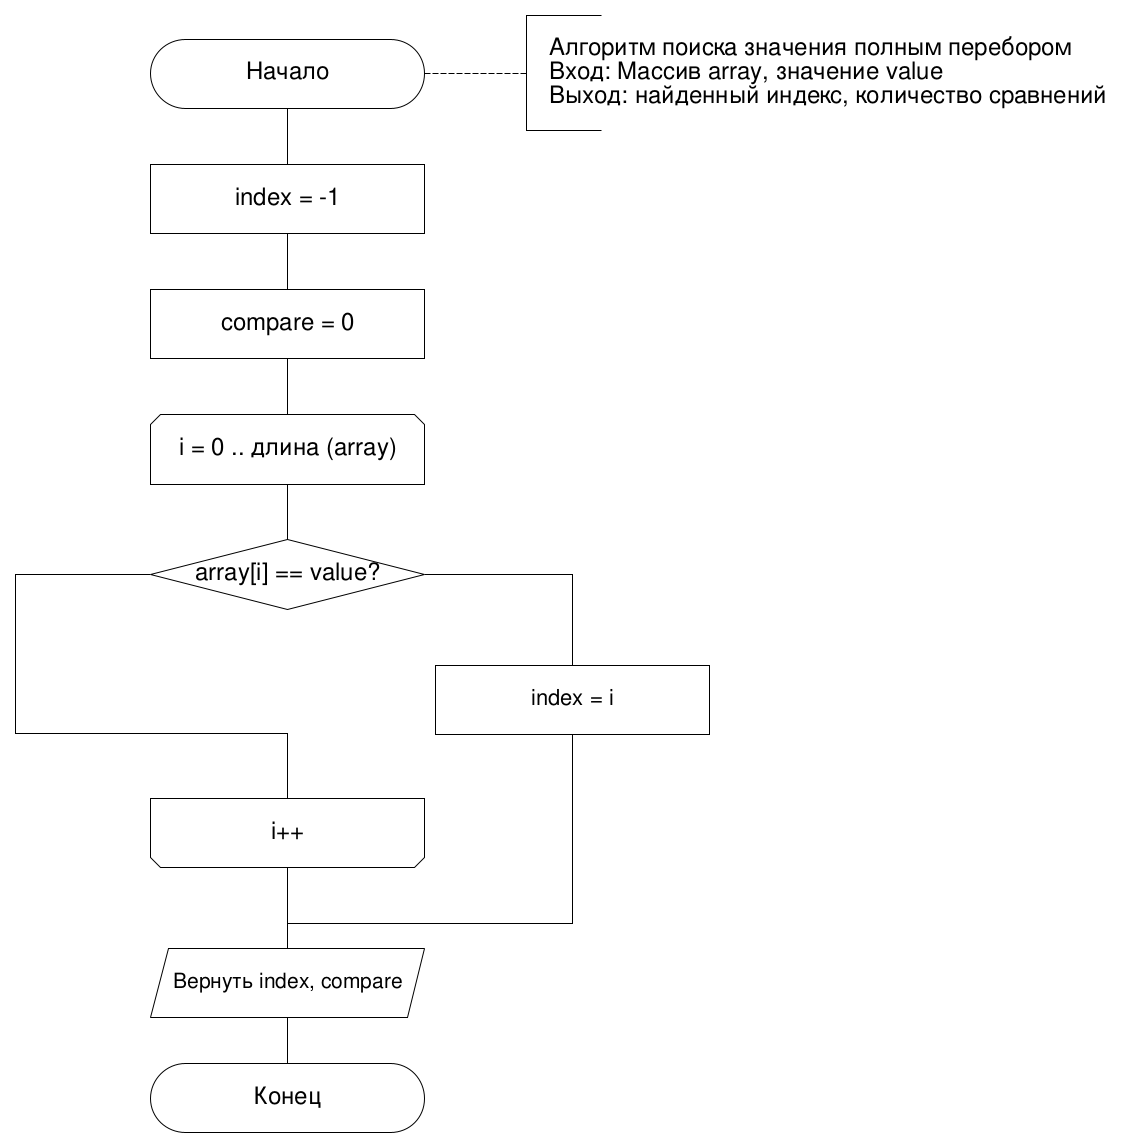
\includegraphics[width=0.8\textwidth]{images/1.png}
    \caption{Схема алгоритма поиска в массиве полным перебором}
    \label{fig:images-1}
\end{figure}

\clearpage

\begin{figure}[h]
    \centering
    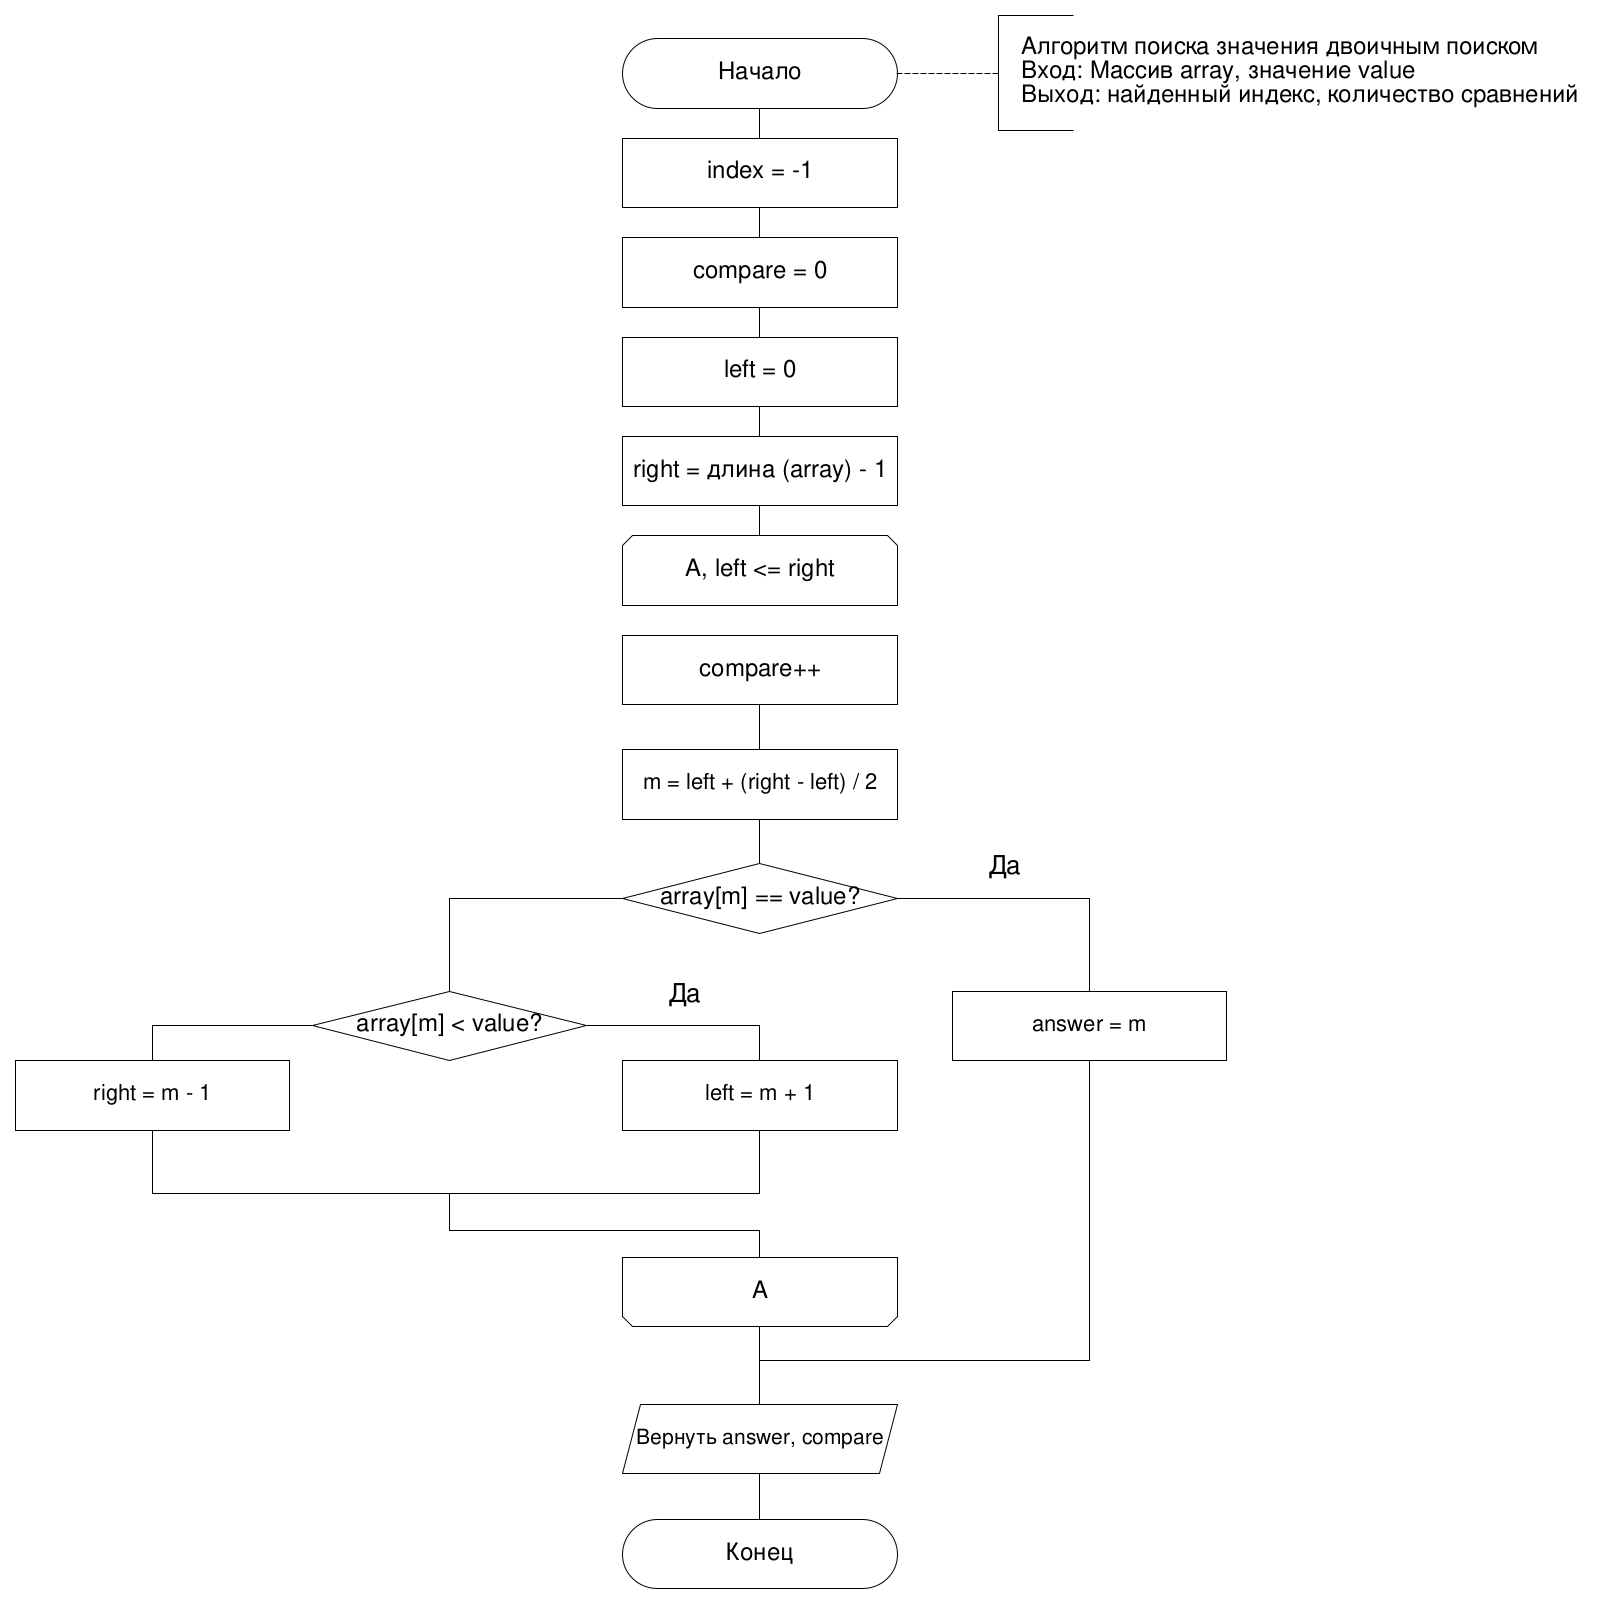
\includegraphics[width=0.8\textwidth]{images/2.png}
    \caption{Схема алгоритма поиска в массиве с помощью двоичного поиска}
    \label{fig:images-2}
\end{figure}

\clearpage

\paragraph*{ВЫВОД} ${}$ \\

В данном разделе были представлены схемы алгоритмов поиска заданного значения в массиве
полным перебором и с помощью двоичного поиска.


\clearpage
